\chapter{METODOLOGI PENELITIAN}

% --- BAGIAN 3.1: WAKTU & TEMPAT (Sesuai Standar Prodi) ---
\section{Waktu, Tempat, dan Jadwal Penelitian}

\subsection{Waktu Pelaksanaan Penelitian}
Penelitian ini dilaksanakan mulai bulan \textbf{[BULAN AWAL TAHUN]} hingga \textbf{[BULAN AKHIR TAHUN]}. Keseluruhan proses penelitian mencakup enam tahapan utama: studi literatur, analisis sistem eksisting, pengumpulan dan preprocessing data, pengembangan model kecerdasan buatan, implementasi sistem, hingga pengujian dan evaluasi performa.

\subsection{Tempat Pelaksanaan Penelitian}
Penelitian ini dilaksanakan di PT Lare Osing Ndo, \textbf{[ALAMAT LENGKAP PERUSAHAAN, KOTA, KODE POS]}. Pengambilan data primer dilakukan secara langsung pada infrastruktur jaringan perusahaan yang terdiri dari \textbf{[JUMLAH]} perangkat aktif (kombinasi Juniper, Huawei, dan MikroTik). Proses pengembangan sistem dilakukan menggunakan workstation portabel (Lenovo ThinkPad T14 Gen 4), sementara proses pelatihan model dilakukan pada lingkungan komputasi lokal dengan spesifikasi yang mendukung operasi pembelajaran mesin.

\subsection{Jadwal Penelitian}
Rincian jadwal kegiatan penelitian disajikan pada Tabel \ref{tab:jadwal_penelitian}. Jadwal ini dirancang secara iteratif mengingat sifat pengembangan sistem berbasis kecerdasan buatan yang memerlukan siklus pengujian dan penyempurnaan berulang.

\begin{table}[H]
    \centering
    \caption{Jadwal Kegiatan Penelitian}
    \label{tab:jadwal_penelitian}
    \begin{tabular}{|c|l|c|c|c|c|c|}
        \hline
        \textbf{No} & \textbf{Kegiatan} & \textbf{Bulan 1} & \textbf{Bulan 2} & \textbf{Bulan 3} & \textbf{Bulan 4} & \textbf{Bulan 5} \\ \hline
        1 & Studi Literatur & \checkmark & & & & \\ \hline
        2 & Analisis Sistem Eksisting & \checkmark & \checkmark & & & \\ \hline
        3 & Pengumpulan Data & & \checkmark & \checkmark & & \\ \hline
        4 & Preprocessing \& Pelabelan & & & \checkmark & & \\ \hline
        5 & Pengembangan Model AI & & & \checkmark & \checkmark & \\ \hline
        6 & Implementasi Sistem & & & & \checkmark & \checkmark \\ \hline
        7 & Pengujian \& Evaluasi & & & & & \checkmark \\ \hline
        8 & Penyusunan Laporan & & & & \checkmark & \checkmark \\ \hline
    \end{tabular}
\end{table}

% --- BAGIAN 3.2: ALAT & BAHAN ---
\section{Alat dan Bahan Penelitian}

Penelitian ini memerlukan kombinasi perangkat keras dan perangkat lunak khusus untuk mendukung pengembangan sistem berbasis pembelajaran mesin pada jaringan komputer. Spesifikasi lengkap alat dan bahan yang digunakan adalah sebagai berikut:

\subsection{Perangkat Keras (\textit{Hardware})}
\begin{enumerate}
    \item \textbf{Workstation Development:}
    \begin{itemize}
        \item Model: Lenovo ThinkPad T14 Gen 4
        \item Processor: Intel Core i7-1370P (13th Gen) dengan 20 logical cores
        \item Graphics: Intel Iris Xe Graphics (RPL-P)
        \item Memory: 32 GB RAM
        \item OS: Fedora Linux 43 (Workstation Edition) dengan kernel 6.17.12
        \item \textit{Windowing System}: Wayland
    \end{itemize}
    Workstation ini digunakan untuk seluruh proses pengembangan, mulai dari pemrograman backend, pengembangan model AI, hingga deployment sistem.

    \item \textbf{Perangkat Jaringan Fisik:}
    \begin{itemize}
        \item Router dan Switch Juniper (JunOS)
        \item Router dan Switch Huawei (VRP Operating System)
        \item Router dan Switch MikroTik (RouterOS)
    \end{itemize}
    Perangkat-perangkat ini merupakan infrastruktur jaringan aktif PT Lare Osing Ndo yang menjadi objek monitoring dan sumber data penelitian.
\end{enumerate}

\subsection{Perangkat Lunak (\textit{Software})}
\begin{enumerate}
    \item \textbf{Backend Development Stack:}
    \begin{itemize}
        \item \textit{Runtime}: Bun (JavaScript/TypeScript runtime yang dioptimasi untuk performa tinggi)
        \item \textit{Web Framework}: Hono (lightweight web framework)
        \item \textit{Database}: PostgreSQL untuk penyimpanan data time-series
        \item \textit{ORM}: Drizzle ORM untuk manajemen database
        \item \textit{SNMP Library}: Net-SNMP untuk polling data perangkat jaringan
    \end{itemize}

    \item \textbf{Machine Learning Development Stack:}
    \begin{itemize}
        \item Bahasa Pemrograman: Python 3.x
        \item \textit{Deep Learning Framework}: PyTorch
        \item \textit{Graph Neural Network Library}: PyTorch Geometric
        \item \textit{API Framework}: FastAPI untuk ML inference service
        \item \textit{Scientific Computing}: NumPy, Pandas untuk manipulasi data
        \item \textit{Graph Processing}: NetworkX untuk analisis graf
        \item \textit{Visualization}: Matplotlib untuk visualisasi hasil training
    \end{itemize}

    \item \textbf{Supporting Tools:}
    \begin{itemize}
        \item Docker untuk kontainerisasi aplikasi
        \item Git untuk version control
        \item \textit{Data Export/Import Tools} terintegrasi dalam sistem frontend
    \end{itemize}
\end{enumerate}

\subsection{Bahan Penelitian}
\begin{enumerate}
    \item \textbf{Data Primer:}
    \begin{itemize}
        \item Data monitoring jaringan real-time yang dikumpulkan melalui protokol SNMP dengan interval polling 1 menit
        \item Data mencakup metrik performa node (CPU usage, RAM usage, total traffic in/out, interface utilization, status)
        \item Data kualitas link (link quality, bandwidth utilization, interface speed, jarak fisik antar node, status koneksi)
        \item Data konfigurasi VLAN dan topologi jaringan layer 2
    \end{itemize}

    \item \textbf{Data Sekunder:}
    \begin{itemize}
        \item Data hasil kuesioner pakar untuk pembobotan kriteria menggunakan metode AHP (\textit{Analytic Hierarchy Process})
        \item Dokumentasi arsitektur jaringan eksisting PT Lare Osing Ndo
    \end{itemize}
\end{enumerate}

% --- BAGIAN 3.3: GAMBARAN SISTEM ---
\section{Gambaran Umum Sistem}

\subsection{Sistem Saat Ini (\textit{Current State})}
Infrastruktur jaringan PT Lare Osing Ndo saat ini menggunakan topologi hybrid dengan kombinasi perangkat dari berbagai vendor (Juniper, Huawei, dan MikroTik). Manajemen lalu lintas data pada layer 2 masih bergantung pada protokol konvensional seperti \textit{Spanning Tree Protocol} (STP) yang bekerja dengan cara memblokir jalur redundan untuk mencegah \textit{broadcast storm}.

Kendala utama dari pendekatan ini antara lain:
\begin{itemize}
    \item Ketidakseimbangan distribusi beban trafik karena STP hanya menggunakan satu jalur aktif
    \item Waktu konvergensi yang lambat (30-50 detik) ketika terjadi kegagalan link
    \item Tidak adanya mekanisme prediktif untuk mengantisipasi degradasi performa jaringan
    \item Konfigurasi manual yang memakan waktu dan rentan \textit{human error}
    \item Keterbatasan visibilitas real-time terhadap kondisi kesehatan jaringan secara menyeluruh
\end{itemize}

\subsection{Sistem yang Diusulkan (\textit{Proposed System})}
Penelitian ini mengusulkan sistem cerdas bernama "\textbf{Laros Watch}" yang mengintegrasikan \textit{Network Management System} (NMS) berbasis SNMP dengan mesin kecerdasan buatan berbasis \textit{Graph Attention Network} (GAT). Sistem ini dirancang untuk memberikan rekomendasi jalur optimal secara real-time dengan mempertimbangkan berbagai metrik performa jaringan secara holistik.

Arsitektur sistem yang diusulkan divisualisasikan pada Gambar \ref{fig:arsitektur_sistem}. Sistem terdiri dari empat layer utama:

\begin{figure}[H]
    \centering
    \includegraphics[width=0.95\textwidth]{images/laros_watch_infra.png}
    \caption{Arsitektur Sistem Laros Watch (Proposed Architecture)}
    \label{fig:arsitektur_sistem}
\end{figure}

\begin{enumerate}
    \item \textbf{Physical Network Layer (Layer Fisik):}

    Layer ini merupakan infrastruktur jaringan fisik tempat perangkat router dan switch beroperasi. Perangkat-perangkat dari vendor Juniper, Huawei, dan MikroTik saling terkoneksi membentuk topologi hybrid. Setiap perangkat dikonfigurasi dengan SNMP agent yang memungkinkan sistem melakukan polling data secara periodik.

    \item \textbf{Data Collection \& Storage Layer:}

    Layer ini bertanggung jawab untuk pengumpulan dan penyimpanan data monitoring. Proses yang terjadi meliputi:
    \begin{itemize}
        \item \textbf{SNMP Polling}: Backend service melakukan polling ke setiap perangkat setiap 1 menit untuk mengambil data real-time
        \item \textbf{Multi-vendor Support}: Sistem mendukung OID (Object Identifier) yang berbeda untuk setiap vendor
        \item \textbf{Data Normalization}: Data mentah dinormalisasi ke range [0,1] untuk memudahkan processing oleh model AI
        \item \textbf{Time-series Storage}: Data disimpan dalam PostgreSQL dengan struktur yang dioptimasi untuk query time-series
    \end{itemize}

    \item \textbf{Core Backend (Application Layer):}

    Layer ini dibangun menggunakan Bun runtime dan Hono framework dengan arsitektur modular yang terdiri dari beberapa service:
    \begin{itemize}
        \item \textbf{SNMP Poller Service}: Mengelola proses polling data dari perangkat jaringan
        \item \textbf{Device Discovery Service}: Melakukan auto-discovery perangkat baru dalam jaringan
        \item \textbf{VLAN Configuration Service}: Mengumpulkan dan mengelola data konfigurasi VLAN
        \item \textbf{Data Aggregation Service}: Mengagregasi data dari berbagai sumber sebelum dikirim ke ML Engine
        \item \textbf{API Gateway}: Menyediakan RESTful API untuk frontend dan integrasi dengan ML Engine
        \item \textbf{Database Layer}: Drizzle ORM untuk manajemen koneksi dan query ke PostgreSQL
    \end{itemize}

    \item \textbf{ML Engine (Intelligence Layer):}

    Layer ini merupakan inti dari sistem kecerdasan buatan yang dibangun menggunakan Python dengan FastAPI sebagai service wrapper. Komponen-komponen utamanya meliputi:
    \begin{itemize}
        \item \textbf{Graph Construction Module}: Mengkonversi data jaringan menjadi representasi graf dengan node (perangkat) dan edge (koneksi)
        \item \textbf{Feature Engineering Module}: Memproses fitur-fitur node (6 dimensi: CPU, RAM, traffic in/out, utilization, status) dan fitur edge (7 dimensi: link quality, bandwidth utilization A/B, interface speed A/B, distance, status)
        \item \textbf{GAT Inference Engine}: Model GAT yang sudah dilatih melakukan forward pass untuk menghasilkan node embeddings
        \item \textbf{Path Recommendation Module}: Menggunakan embeddings untuk menghitung skor kualitas setiap kemungkinan jalur dan memberikan Top-K rekomendasi
        \item \textbf{AHP Weighting Module}: Menerapkan bobot preferensi dari hasil kuesioner pakar
    \end{itemize}

    \item \textbf{Presentation Layer (Frontend):}

    Layer antarmuka pengguna yang menampilkan visualisasi topologi jaringan, status real-time perangkat, rekomendasi jalur optimal, serta menyediakan fitur export data untuk keperluan re-training model.
\end{enumerate}

\subsection{Alur Kerja Sistem}
Sistem Laros Watch beroperasi dengan alur kerja sebagai berikut:
\begin{enumerate}
    \item Backend melakukan polling SNMP ke seluruh perangkat setiap 1 menit
    \item Data yang terkumpul disimpan ke database PostgreSQL
    \item Ketika terjadi perubahan status node atau link, atau saat user meminta rekomendasi jalur, backend mengirim snapshot data terkini ke ML Engine melalui REST API
    \item ML Engine mengkonversi data menjadi struktur graf PyTorch Geometric
    \item Model GAT melakukan inferensi untuk menghasilkan node embeddings
    \item Algoritma path recommendation menghitung skor kualitas untuk semua jalur yang mungkin
    \item Top-K jalur terbaik dikembalikan ke backend
    \item Frontend menampilkan hasil rekomendasi kepada network administrator
    \item Administrator dapat menggunakan informasi ini untuk melakukan routing decision atau konfigurasi VLAN secara manual/otomatis
\end{enumerate}

% --- BAGIAN 3.4: TAHAPAN PENELITIAN ---
\section{Tahapan Penelitian}

Penelitian ini dirancang mengikuti metodologi penelitian kuantitatif dengan pendekatan eksperimental. Alur penelitian secara umum mengikuti kerangka kerja \textit{Machine Learning Development Lifecycle} yang divisualisasikan pada Gambar \ref{fig:alur_penelitian}.

\begin{figure}[H]
    \centering
    \includegraphics[width=0.7\textwidth]{images/flowchart3.png}
    \caption{Diagram Alur Metodologi Penelitian}
    \label{fig:alur_penelitian}
\end{figure}

Setiap tahapan penelitian dijelaskan secara rinci sebagai berikut:

\subsection{Tahap 1: Identifikasi Masalah dan Studi Literatur}
Tahap awal penelitian dimulai dengan identifikasi masalah pada sistem manajemen jaringan eksisting PT Lare Osing Ndo. Permasalahan utama yang teridentifikasi adalah keterbatasan protokol STP dalam menangani distribusi beban dan adaptasi terhadap perubahan kondisi jaringan secara dinamis.

Studi literatur dilakukan untuk mengkaji:
\begin{itemize}
    \item State-of-the-art dalam \textit{intelligent network management}
    \item Aplikasi \textit{Graph Neural Networks} untuk optimasi routing
    \item Metode \textit{multi-criteria decision making} seperti AHP
    \item Protokol monitoring jaringan (SNMP, NetFlow, sFlow)
    \item Best practices dalam implementasi sistem NMS
\end{itemize}

\subsection{Tahap 2: Perancangan Arsitektur Sistem}
Berdasarkan hasil analisis masalah dan studi literatur, dirancang arsitektur sistem Laros Watch yang mencakup:
\begin{itemize}
    \item Desain database schema untuk time-series data
    \item Perancangan API endpoints untuk komunikasi antar service
    \item Definisi struktur graf untuk representasi topologi jaringan
    \item Perancangan arsitektur model GAT yang sesuai dengan karakteristik data
\end{itemize}

\subsection{Tahap 3: Implementasi Backend dan Data Collection}
Tahap ini melibatkan pengembangan core backend system menggunakan Bun dan Hono framework. Implementasi mencakup:
\begin{itemize}
    \item Pengembangan SNMP polling service dengan dukungan multi-vendor (Juniper, Huawei, MikroTik)
    \item Implementasi device discovery mechanism
    \item Setup PostgreSQL database dengan Drizzle ORM
    \item Pengembangan REST API untuk frontend dan ML Engine
    \item Testing konektivitas dan akurasi pengambilan data dari perangkat fisik
\end{itemize}

\subsection{Tahap 4: Pengumpulan dan Preprocessing Data}
Data monitoring dikumpulkan dari jaringan operasional PT Lare Osing Ndo. Proses yang dilakukan:
\begin{itemize}
    \item Pengumpulan data historis untuk periode minimal 2-4 minggu
    \item Cleaning data (handling missing values, outlier detection)
    \item Normalisasi data menggunakan Min-Max scaling ke range [0,1]
    \item Konversi data tabular menjadi struktur graf (nodes dan edges)
    \item Export data ke format CSV dan PyTorch Geometric Data untuk keperluan training
\end{itemize}

\subsection{Tahap 5: Pelabelan Data dengan AHP}
Karena tidak tersedia ground truth untuk "jalur optimal", dilakukan pelabelan menggunakan metode AHP:
\begin{itemize}
    \item Penyusunan kuesioner AHP untuk \textit{network engineer} senior
    \item Perhitungan bobot kriteria dengan memastikan \textit{Consistency Ratio} (CR) $\leq$ 0.1
    \item Implementasi algoritma Dijkstra termodifikasi dengan cost function berbasis AHP
    \item Generate skor kualitas jalur untuk training dataset
\end{itemize}

\subsection{Tahap 6: Pengembangan dan Pelatihan Model AI}
Tahap ini merupakan inti dari penelitian, dijelaskan lebih detail pada bagian \ref{sec:pengembangan_model}.

\subsection{Tahap 7: Integrasi Sistem}
Setelah model terlatih dengan baik, dilakukan integrasi antara backend, ML Engine, dan frontend:
\begin{itemize}
    \item Deployment model GAT sebagai FastAPI service
    \item Implementasi API call dari backend ke ML Engine
    \item Testing end-to-end system flow
    \item Performance optimization (caching, async processing)
\end{itemize}

\subsection{Tahap 8: Pengujian dan Evaluasi}
Tahap final mencakup pengujian komprehensif sistem dengan berbagai skenario (dijelaskan pada bagian \ref{sec:pengujian}).

% --- BAGIAN 3.5: PENGUMPULAN DATA ---
\section{Metode Pengumpulan Data}

\subsection{Jenis Data yang Dikumpulkan}
Penelitian ini menggunakan dua kategori data utama:

\subsubsection{Data Kuantitatif (SNMP Monitoring Data)}
Data kuantitatif dikumpulkan secara otomatis melalui protokol SNMP dengan interval polling 1 menit. Sistem mendukung pengambilan data dari berbagai vendor dengan mapping OID yang telah dikonfigurasi.

\textbf{Data Level Node (Device-level Metrics):}
\begin{enumerate}
    \item \textbf{Identifikasi Perangkat:}
    \begin{itemize}
        \item System Name (sysName.0: 1.3.6.1.2.1.1.5.0)
        \item System Description (sysDescr.0: 1.3.6.1.2.1.1.1.0)
        \item System Object ID untuk vendor detection
    \end{itemize}

    \item \textbf{Metrik Performa:}
    \begin{itemize}
        \item CPU Usage (\%) - dinormalisasi ke [0,1]
        \item RAM Usage (\%) - dinormalisasi ke [0,1]
        \item Total Traffic In (octets) - dinormalisasi
        \item Total Traffic Out (octets) - dinormalisasi
        \item Average Interface Utilization (\%) - dinormalisasi ke [0,1]
        \item Device Reachability Status (binary: 0=down, 1=up)
    \end{itemize}
\end{enumerate}

\textbf{Data Level Edge (Link-level Metrics):}
\begin{enumerate}
    \item \textbf{Informasi Interface:}
    \begin{itemize}
        \item Interface Index (ifIndex)
        \item Interface Name/Description (ifName, ifDescr)
        \item Interface Type (ifType: Ethernet, FastEthernet, GigabitEthernet, dll)
        \item MAC Address (ifPhysAddress)
    \end{itemize}

    \item \textbf{Metrik Link Quality:}
    \begin{itemize}
        \item Link Quality Score (gabungan dari error rate dan signal strength) - [0,1]
        \item Bandwidth Utilization Interface A (\%) - [0,1]
        \item Bandwidth Utilization Interface B (\%) - [0,1]
        \item Interface Speed A (Mbps/Gbps) - dinormalisasi
        \item Interface Speed B (Mbps/Gbps) - dinormalisasi
        \item Physical Distance (meter) - dinormalisasi berdasarkan jarak maksimal dalam jaringan
        \item Link Status (operational status: up/down) - binary [0,1]
    \end{itemize}

    \item \textbf{Data Optik (untuk SFP/SFP+ modules):}
    \begin{itemize}
        \item Tx Power (dBm)
        \item Rx Power (dBm)
    \end{itemize}

    \item \textbf{Statistik Trafik:}
    \begin{itemize}
        \item Octets In/Out
        \item Unicast Packets In/Out
        \item Error Packets
    \end{itemize}
\end{enumerate}

\textbf{Data Konfigurasi VLAN:}
\begin{itemize}
    \item VLAN ID
    \item VLAN Name
    \item Tagged/Untagged Port Membership
    \item Port VLAN ID (PVID)
\end{itemize}

\subsubsection{Data Kualitatif (Expert Judgment)}
Data kualitatif diperoleh melalui kuesioner AHP yang diisi oleh network engineer senior PT Lare Osing Ndo. Kuesioner dirancang untuk menangkap preferensi relatif terhadap kriteria pemilihan jalur optimal, mencakup:
\begin{itemize}
    \item Bobot preferensi untuk metrik node (CPU score, RAM score, traffic score, utilization score, status)
    \item Bobot preferensi untuk metrik edge (link quality, bandwidth utilization, interface speed, distance, status)
    \item Bobot preferensi untuk komponen routing (link quality, bandwidth utilization, distance)
\end{itemize}

\subsection{Prosedur Pengumpulan Data}

\subsubsection{Pengumpulan Data SNMP}
\begin{enumerate}
    \item \textbf{Konfigurasi SNMP Agent:}

    Setiap perangkat jaringan dikonfigurasi dengan SNMP v2c atau v3 dengan community string yang aman. Akses dibatasi hanya untuk IP address sistem monitoring.

    \item \textbf{Device Discovery:}

    Sistem melakukan auto-discovery perangkat menggunakan kombinasi teknik:
    \begin{itemize}
        \item Ping sweep pada subnet yang telah ditentukan
        \item SNMP walk untuk mengidentifikasi perangkat yang merespon
        \item MAC address table parsing untuk menemukan perangkat terkoneksi
        \item LLDP (Link Layer Discovery Protocol) untuk mendapatkan informasi neighbor
    \end{itemize}

    \item \textbf{Polling Mechanism:}

    Backend service menjalankan scheduled task setiap 1 menit untuk melakukan SNMP GET request ke setiap perangkat. Implementasi menggunakan async/await pattern untuk memaksimalkan throughput:

    \begin{verbatim}
    async function pollAllDevices() {
        const devices = await db.select().from(deviceTable);
        const pollPromises = devices.map(device =>
            pollSingleDevice(device)
        );
        await Promise.allSettled(pollPromises);
    }
    \end{verbatim}

    \item \textbf{Error Handling:}

    Sistem menangani berbagai kondisi error seperti timeout, unreachable device, dan invalid OID dengan retry mechanism dan logging untuk troubleshooting.

    \item \textbf{Data Validation:}

    Data yang terkumpul divalidasi untuk memastikan konsistensi (misalnya: interface speed tidak boleh 0, utilization tidak boleh > 100\%).
\end{enumerate}

\subsubsection{Pengumpulan Data AHP}
\begin{enumerate}
    \item Penyusunan kuesioner berdasarkan kriteria yang relevan dengan kualitas jalur jaringan
    \item Koordinasi dengan network engineer senior untuk pengisian kuesioner
    \item Pengolahan hasil kuesioner menggunakan metode AHP standar
    \item Validasi konsistensi dengan menghitung Consistency Ratio (CR)
    \item Jika CR > 0.1, dilakukan revisi dan pengisian ulang kuesioner
    \item Export hasil pembobotan ke file JSON untuk digunakan dalam training model
\end{enumerate}

\subsection{Normalisasi Data}
Seluruh data numerik dinormalisasi menggunakan Min-Max scaling untuk memastikan semua fitur berada dalam range yang sama:

\begin{equation}
x_{norm} = \frac{x - x_{min}}{x_{max} - x_{min}}
\end{equation}

Untuk metrik yang bersifat "lower is better" seperti CPU usage dan latency, dilakukan inversi:

\begin{equation}
x_{inverted} = 1 - x_{norm}
\end{equation}

% --- BAGIAN 3.6: PENGEMBANGAN MODEL ---
\section{Metode Pengembangan Model AI}
\label{sec:pengembangan_model}

Pengembangan model kecerdasan buatan dalam penelitian ini mengikuti kerangka kerja \textit{Machine Learning Pipeline} yang divisualisasikan pada Gambar \ref{fig:model_pipeline}. Berbeda dengan pengembangan aplikasi konvensional, pengembangan model AI memerlukan proses iteratif yang mencakup data preparation, model architecture design, training, dan evaluation.

\begin{figure}[H]
    \centering
    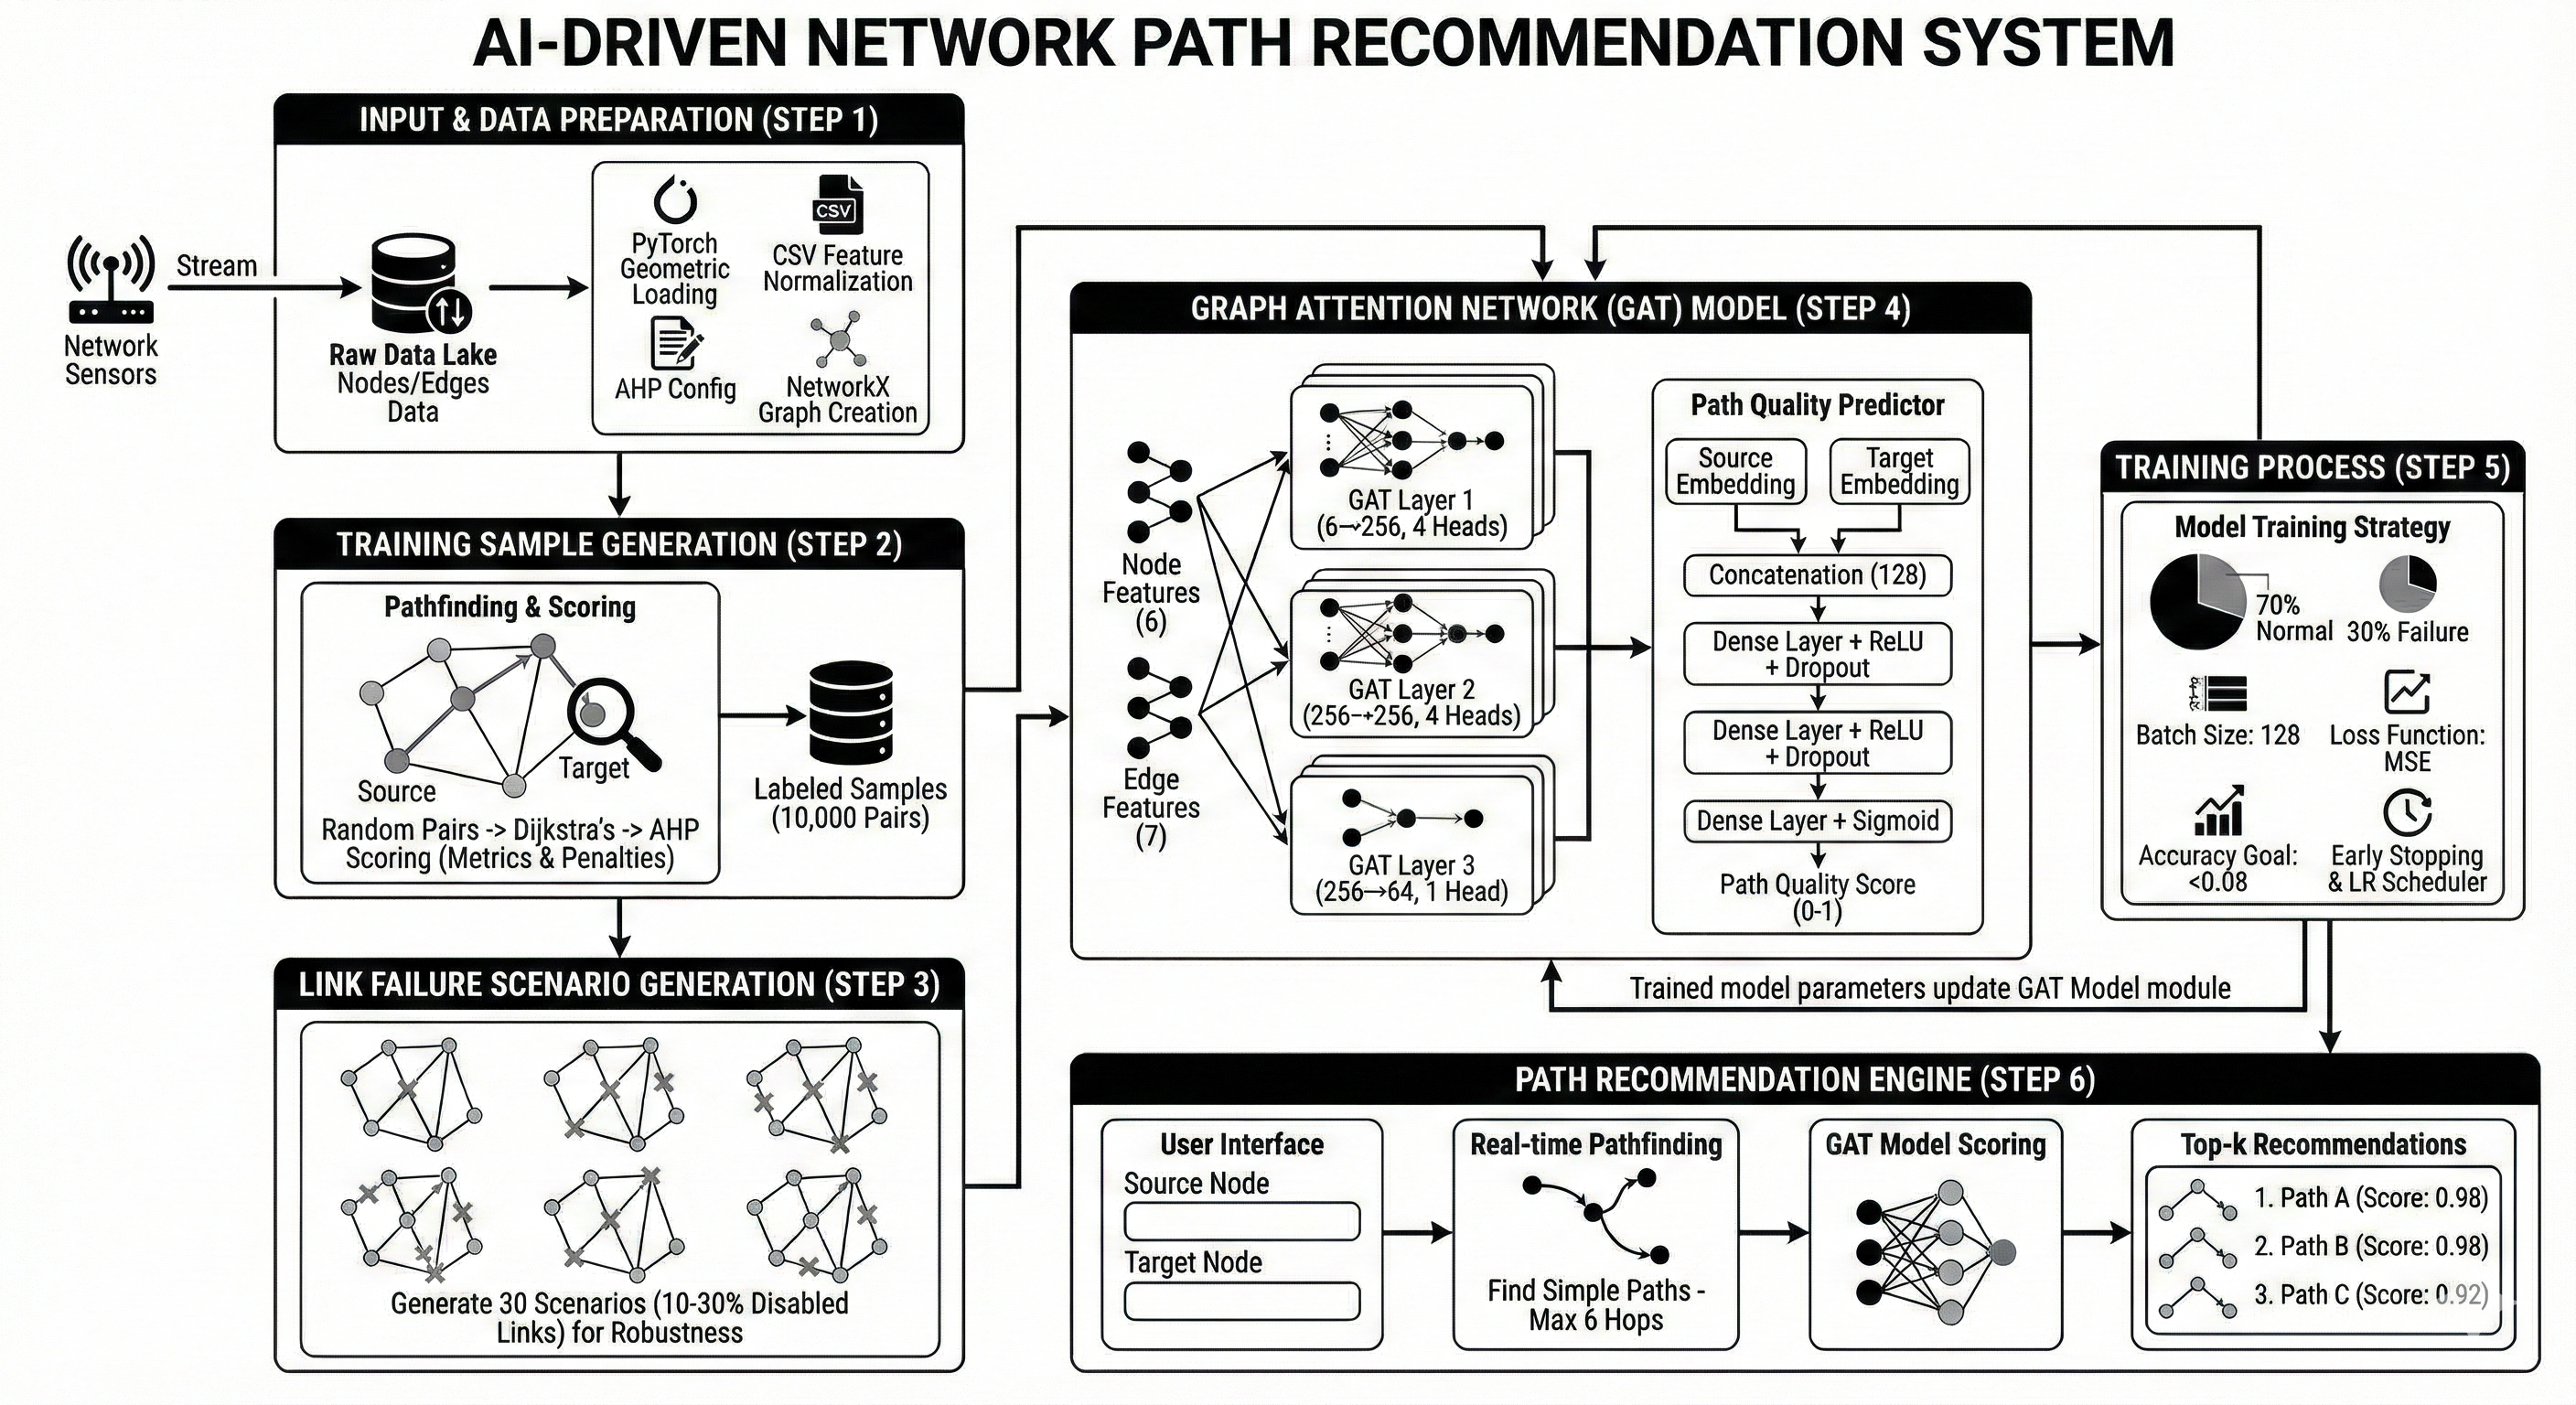
\includegraphics[width=1.0\textwidth]{images/model_flow.png}
    \caption{Alur Pengembangan dan Pelatihan Model GAT}
    \label{fig:model_pipeline}
\end{figure}

\subsection{Step 1 \& 2: Persiapan Data dan Pelabelan}

\subsubsection{Loading dan Konversi Data}
Data yang telah dinormalisasi dimuat ke dalam format PyTorch Geometric Data object yang merepresentasikan graf jaringan:

\begin{itemize}
    \item \textbf{Node Features} ($\mathbf{X} \in \mathbb{R}^{N \times 6}$): Matrix berisi 6 fitur untuk setiap node (CPU usage, RAM usage, traffic in, traffic out, interface utilization, status)
    \item \textbf{Edge Index} ($\mathbf{E} \in \mathbb{Z}^{2 \times M}$): Adjacency list format yang merepresentasikan koneksi antar node
    \item \textbf{Edge Features} ($\mathbf{E}_{attr} \in \mathbb{R}^{M \times 7}$): Matrix berisi 7 fitur untuk setiap edge
\end{itemize}

\subsubsection{Pelabelan dengan AHP-Enhanced Dijkstra}
Karena tidak ada ground truth untuk "jalur optimal", penelitian ini menggunakan pendekatan domain expert melalui AHP. Proses pelabelan dilakukan sebagai berikut:

\begin{enumerate}
    \item \textbf{Perhitungan Bobot AHP:}

    Dari kuesioner pakar, diperoleh bobot untuk setiap kriteria. Contoh konfigurasi bobot:
    \begin{verbatim}
    edge_routing_weights = {
        "link_quality": 0.538,
        "bandwidth_util": 0.297,
        "distance": 0.165
    }
    \end{verbatim}

    \item \textbf{Konstruksi Graf Berbobot:}

    Setiap edge dalam graf diberi bobot cost berdasarkan formula:
    \begin{equation}
    w_{edge} = (1 - q_{link}) \cdot w_{LQ} + u_{bw} \cdot w_{BW} + d_{norm} \cdot w_{D}
    \end{equation}
    dimana:
    \begin{itemize}
        \item $q_{link}$: Link quality score [0,1]
        \item $u_{bw}$: Bandwidth utilization [0,1]
        \item $d_{norm}$: Normalized distance [0,1]
        \item $w_{LQ}, w_{BW}, w_{D}$: Bobot AHP dari expert judgment
     \end{itemize}
     \item \textbf{Perhitungan Skor Kualitas Node:}

         Skor kualitas untuk setiap node dihitung menggunakan formula:
         \begin{equation}
         Q_{node} = \sum_{i=1}^{5} (1 - f_i) \cdot w_i
         \end{equation}
         dimana $f_i$ adalah fitur yang sudah dinormalisasi (CPU, RAM, traffic, utilization) dan $w_i$ adalah bobot AHP. Inversi (1 - $f_i$) dilakukan karena nilai rendah menandakan kualitas lebih baik.

         \item \textbf{Perhitungan Skor Kualitas Edge:}

         Untuk setiap edge, skor dihitung dengan:
         \begin{equation}
         Q_{edge} = q_{link} \cdot w_1 + (1 - u_{bw,A}) \cdot w_2 + (1 - u_{bw,B}) \cdot w_3 + s_A \cdot w_4 + s_B \cdot w_5 + (1 - d) \cdot w_6 + st \cdot w_7
         \end{equation}
         dimana $s_A, s_B$ adalah interface speed, $st$ adalah status link, dan $w_1...w_7$ adalah bobot AHP.

         \item \textbf{Perhitungan Skor Kualitas Jalur:}

         Untuk sebuah jalur $P = \{v_1, v_2, ..., v_k\}$, skor kualitas total dihitung sebagai:
         \begin{equation}
         Q_{path} = \left( \frac{\sum_{i=1}^{k} Q_{node}(v_i) + \sum_{j=1}^{k-1} Q_{edge}(e_j)}{2k-1} \right) \times (1 - \alpha \cdot h)
         \end{equation}
         dimana:
         \begin{itemize}
             \item $k$: jumlah node dalam jalur
             \item $h = k - 1$: jumlah hop
             \item $\alpha = 0.05$: faktor penalti hop (hop penalty factor)
         \end{itemize}

         Hop penalty diterapkan karena jalur yang lebih panjang cenderung memiliki latency lebih tinggi dan risiko kegagalan lebih besar.
     \end{enumerate}

     \subsubsection{Generasi Training Samples}
     Untuk memaksimalkan pembelajaran model, training dataset di-generate dengan strategi yang mencakup variasi kualitas jalur:

     \begin{enumerate}
         \item \textbf{Optimal Paths (60\%):} Jalur yang dipilih oleh algoritma Dijkstra dengan cost function berbasis AHP. Jalur-jalur ini merepresentasikan keputusan routing terbaik berdasarkan expert judgment.

         \item \textbf{Alternative Paths (40\%):} Jalur-jalur alternatif yang lebih panjang atau melewati link dengan kualitas lebih rendah. Ini penting agar model belajar membedakan jalur berkualitas tinggi vs rendah.
     \end{enumerate}

     Total 10,000 training samples di-generate dengan distribusi:
     \begin{itemize}
         \item 6,000 samples optimal paths
         \item 4,000 samples alternative paths
     \end{itemize}

     Setiap sample berisi informasi:
     \begin{itemize}
         \item Source dan target node index
         \item Sequence of nodes dalam jalur
         \item Path length (jumlah hop)
         \item Quality score (label untuk supervised learning)
         \item Path type (optimal/alternative)
     \end{itemize}

     \subsection{Step 3: Skenario Kegagalan Tautan (\textit{Link Failure Scenarios})}

     Untuk meningkatkan robustness model dalam menghadapi kondisi jaringan yang tidak ideal, dilakukan generasi data sintetis dengan simulasi kegagalan link. Pendekatan ini penting karena dalam operasional nyata, jaringan sering mengalami gangguan parsial.

     \subsubsection{Prosedur Generasi Failure Scenarios}
     \begin{enumerate}
         \item Dari graf topologi original, dibuat 30 skenario kegagalan yang berbeda
         \item Setiap skenario menonaktifkan 10-30\% edge secara random
         \item Edge yang dinonaktifkan dipilih menggunakan random sampling tanpa replacement
         \item Setiap skenario disimpan sebagai modified PyTorch Geometric Data object
     \end{enumerate}

     \subsubsection{Distribusi Failure Scenarios}
     \begin{table}[H]
         \centering
         \caption{Distribusi Skenario Kegagalan Link}
         \begin{tabular}{|c|c|c|}
             \hline
             \textbf{Kategori} & \textbf{Persentase Link Disabled} & \textbf{Jumlah Skenario} \\ \hline
             Minor Failure & 10-15\% & 10 \\ \hline
             Moderate Failure & 15-25\% & 12 \\ \hline
             Major Failure & 25-30\% & 8 \\ \hline
         \end{tabular}
     \end{table}

     \subsubsection{Tujuan Failure Scenarios}
     \begin{itemize}
         \item Melatih model untuk beradaptasi dengan perubahan topologi
         \item Menghindari overfitting pada topologi statis
         \item Meningkatkan kemampuan generalisasi model
         \item Mensimulasikan kondisi real-world dimana link bisa gagal sewaktu-waktu
     \end{itemize}

     Selama training, model akan bergantian dilatih menggunakan:
     \begin{itemize}
         \item Graf normal (topologi lengkap) - untuk belajar routing optimal
         \item Graf dengan failure scenarios - untuk belajar failover routing
     \end{itemize}

     \subsection{Step 4: Arsitektur Graph Attention Network (GAT)}

     Model yang digunakan dalam penelitian ini adalah \textit{Graph Attention Network} (GAT), sebuah arsitektur \textit{Graph Neural Network} yang menggunakan mekanisme attention untuk memberikan bobot berbeda pada tetangga setiap node. Arsitektur ini dipilih karena kemampuannya dalam menangkap struktur graf yang kompleks dan heterogen seperti topologi jaringan komputer.

     \subsubsection{Arsitektur Layer-by-Layer}

     Model GAT dalam penelitian ini terdiri dari tiga layer GAT dengan konfigurasi sebagai berikut:

     \begin{enumerate}
         \item \textbf{GAT Layer 1 (Input Layer):}
         \begin{itemize}
             \item Input dimension: 6 (node features)
             \item Output dimension: 64
             \item Number of attention heads: 4
             \item Total output dimension: 64 × 4 = 256
             \item Edge dimension: 7 (edge features digunakan dalam attention mechanism)
             \item Activation: ELU (Exponential Linear Unit)
             \item Dropout: 0.3
         \end{itemize}

         Formula attention untuk layer 1:
         \begin{equation}
         \mathbf{h}_i^{(1)} = \|_{k=1}^{4} \sigma \left( \sum_{j \in \mathcal{N}(i)} \alpha_{ij}^k \mathbf{W}^k \mathbf{h}_j^{(0)} \right)
         \end{equation}
         dimana $\alpha_{ij}^k$ adalah attention weight untuk head ke-$k$, $\mathbf{W}^k$ adalah weight matrix, dan $\|$ adalah concatenation operator.

         \item \textbf{GAT Layer 2 (Hidden Layer):}
         \begin{itemize}
             \item Input dimension: 256 (dari layer 1)
             \item Output dimension: 64
             \item Number of attention heads: 4
             \item Total output dimension: 64 × 4 = 256
             \item Edge dimension: 7
             \item Activation: ELU
             \item Dropout: 0.3
         \end{itemize}

         Layer ini berfungsi untuk memperdalam representasi dengan menangkap pola interaksi yang lebih kompleks antar node dalam radius 2-hop neighborhood.

         \item \textbf{GAT Layer 3 (Output Layer):}
         \begin{itemize}
             \item Input dimension: 256 (dari layer 2)
             \item Output dimension: 64
             \item Number of attention heads: 1 (single head untuk agregasi final)
             \item Total output dimension: 64
             \item Edge dimension: 7
             \item Activation: Linear (no activation, raw embeddings)
             \item Dropout: 0.3
         \end{itemize}

         Layer final menghasilkan node embeddings dengan dimensi 64 yang merepresentasikan karakteristik setiap node dalam konteks graf.
     \end{enumerate}

     \subsubsection{Path Quality Predictor}

     Setelah GAT layers menghasilkan node embeddings, digunakan \textit{Path Quality Predictor} - sebuah feed-forward neural network untuk memprediksi skor kualitas jalur:

     \begin{itemize}
         \item \textbf{Input:} Concatenation dari embeddings source dan target node untuk setiap hop → dimensi: 64 + 64 = 128
         \item \textbf{Hidden Layer 1:} Linear(128 → 128) + ReLU + Dropout(0.3)
         \item \textbf{Hidden Layer 2:} Linear(128 → 64) + ReLU + Dropout(0.3)
         \item \textbf{Output Layer:} Linear(64 → 1) + Sigmoid
         \item \textbf{Output:} Quality score dalam range [0, 1]
     \end{itemize}

     Formula prediksi untuk single hop:
     \begin{equation}
     q_{hop}(i,j) = \sigma \left( \mathbf{W}_3 \cdot \text{ReLU}(\mathbf{W}_2 \cdot \text{ReLU}(\mathbf{W}_1 \cdot [\mathbf{h}_i || \mathbf{h}_j])) \right)
     \end{equation}

     Untuk jalur lengkap $P = \{v_1, v_2, ..., v_k\}$, skor total dihitung dengan:
     \begin{equation}
     Q_{path} = \left( \frac{1}{k-1} \sum_{i=1}^{k-1} q_{hop}(v_i, v_{i+1}) \right) \times (1 - 0.03 \cdot (k-1))
     \end{equation}

     \subsubsection{Justifikasi Pemilihan Hyperparameters}

     \begin{itemize}
         \item \textbf{Hidden dimension 64:} Dipilih berdasarkan trade-off antara kapasitas model dan computational cost. Dimensi ini cukup untuk menangkap kompleksitas jaringan \textbf{[JUMLAH]} node tanpa overfitting.

         \item \textbf{4 attention heads:} Multi-head attention memungkinkan model belajar berbagai aspek relasi antar node secara paralel (misalnya: proximity, bandwidth similarity, load balance).

         \item \textbf{3 layers:} Memberikan receptive field 3-hop, artinya setiap node bisa "melihat" informasi dari node-node dalam radius 3 hop. Ini mencukupi untuk jaringan dengan diameter relatif kecil.

         \item \textbf{Dropout 0.3:} Regularisasi untuk mencegah overfitting, terutama penting karena model dilatih dengan data sintetis (failure scenarios).

         \item \textbf{ELU activation:} Memberikan performa lebih baik dibanding ReLU untuk graph neural networks karena smooth gradient untuk nilai negatif.
     \end{itemize}

     \subsubsection{Total Parameters}
     Model memiliki total \textbf{approximately 500,000} trainable parameters, yang terdistribusi di:
     \begin{itemize}
         \item GAT layers: ~350,000 parameters
         \item Path predictor MLP: ~150,000 parameters
     \end{itemize}

     \subsection{Step 5: Strategi Pelatihan Model}

     Proses pelatihan model dirancang dengan strategi khusus untuk mengoptimalkan performa pada task path recommendation dalam konteks jaringan yang dinamis.

     \subsubsection{Konfigurasi Training}

     \begin{table}[H]
         \centering
         \caption{Hyperparameter Training}
         \begin{tabular}{|l|l|}
             \hline
             \textbf{Parameter} & \textbf{Value} \\ \hline
             Optimizer & Adam \\ \hline
             Initial Learning Rate & 0.001 \\ \hline
             Weight Decay & 5e-4 \\ \hline
             Loss Function & Mean Squared Error (MSE) \\ \hline
             Batch Size & 128 samples \\ \hline
             Max Epochs & 1000 \\ \hline
             Early Stopping Patience & 25 epochs \\ \hline
             Gradient Clipping & Max norm = 1.0 \\ \hline
             Train/Val Split & 80\% / 20\% \\ \hline
             Device & CPU (Intel i7-1370P) \\ \hline
         \end{tabular}
     \end{table}

     \subsubsection{Loss Function}

     Model dilatih menggunakan Mean Squared Error (MSE) antara predicted quality score dan true quality score (dari AHP):

     \begin{equation}
     \mathcal{L}_{MSE} = \frac{1}{N} \sum_{i=1}^{N} (Q_{pred}^{(i)} - Q_{true}^{(i)})^2
     \end{equation}

     MSE dipilih karena:
     \begin{itemize}
         \item Sesuai untuk regression task (prediksi skor kontinyu)
         \item Memberikan penalti lebih besar untuk error yang besar
         \item Smooth gradient untuk optimasi
     \end{itemize}

     \subsubsection{Learning Rate Scheduling}

     Penelitian ini menggunakan \textit{Cosine Annealing with Warm Restarts} untuk learning rate scheduling:

     \begin{equation}
     \eta_t = \eta_{min} + \frac{1}{2}(\eta_{max} - \eta_{min})(1 + \cos(\frac{T_{cur}}{T_i}\pi))
     \end{equation}

     Parameter scheduling:
     \begin{itemize}
         \item $T_0 = 20$ epochs (periode restart pertama)
         \item $T_{mult} = 2$ (periode restart dikali 2 setiap restart)
         \item $\eta_{min} = 1e-6$ (minimum learning rate)
     \end{itemize}

     Scheduling ini memungkinkan model "escape" dari local minima dengan periodic restart pada learning rate yang lebih tinggi.

     \subsubsection{Alternating Training Strategy}

     Untuk melatih model yang robust terhadap failure, digunakan strategi alternating training:

     \begin{verbatim}
     Algorithm: Alternating Training with Failure Scenarios
     -------------------------------------------------------
     FOR epoch = 1 to max_epochs:
         IF epoch mod (num_scenarios + 1) == 0:
             current_graph = normal_graph
         ELSE:
             scenario_idx = epoch mod (num_scenarios + 1) - 1
             current_graph = failure_scenarios[scenario_idx]

         embeddings = model.forward(current_graph)
         batch_samples = sample_training_data(valid_paths_only)
         loss = compute_loss(embeddings, batch_samples)
         loss.backward()
         optimizer.step()
     \end{verbatim}

     Strategi ini memastikan model terpapar dengan:
     \begin{itemize}
         \item Kondisi normal (1/31 epochs)
         \item Berbagai kondisi failure (30/31 epochs)
     \end{itemize}

     \subsubsection{Data Composition Strategy}

     Untuk setiap epoch, training batch terdiri dari:
     \begin{itemize}
         \item 70\% samples dari kondisi normal
         \item 30\% samples dari kondisi failure
     \end{itemize}

     Komposisi ini berdasarkan asumsi bahwa dalam operasional nyata:
     \begin{itemize}
         \item Jaringan mayoritas berada dalam kondisi normal
         \item Failure events terjadi secara sporadis
         \item Model harus tetap perform optimal pada kondisi normal
         \item Model harus adaptif ketika failure terjadi
     \end{itemize}

     \subsubsection{Early Stopping Mechanism}

     Untuk mencegah overfitting, diterapkan early stopping dengan kriteria:

     \begin{itemize}
         \item Monitor: Validation loss
         \item Patience: 25 epochs tanpa improvement
         \item Improvement threshold: 0.5\% reduction in validation loss ATAU 1\% increase in validation accuracy
         \item Best model: Disimpan berdasarkan validation loss terendah
     \end{itemize}

     \subsubsection{Gradient Clipping}

     Untuk stabilitas training, diterapkan gradient clipping dengan threshold $\tau = 1.0$ untuk mencegah exploding gradients yang sering terjadi pada graph neural networks.

     \subsubsection{Validation Strategy}

     Validation dilakukan setiap epoch dengan:
     \begin{itemize}
         \item Validation set: 20\% dari total samples (2,000 samples)
         \item Evaluation menggunakan graf normal (bukan failure scenarios)
         \item Metrik yang di-track: Validation Loss (MSE) dan Validation Accuracy dengan tolerance $\pm$0.05, $\pm$0.08, $\pm$0.10
     \end{itemize}

     \subsection{Step 6: Testing dan Inferensi}

     Setelah model terlatih, dilakukan testing untuk memvalidasi kemampuan model dalam memberikan rekomendasi jalur pada kondisi real-time.

     \subsubsection{Inference Pipeline}

     Proses inferensi mengikuti langkah berikut:

     \begin{enumerate}
         \item \textbf{Input Preparation:} Load current network state, specify source dan target node
         \item \textbf{Graph Processing:} Convert ke NetworkX graph, filter edge aktif, compute shortest path
         \item \textbf{Path Generation:} Enumerate semua jalur dengan dynamic cutoff
         \item \textbf{Quality Scoring:} Forward pass model untuk node embeddings, hitung skor setiap jalur
         \item \textbf{Ranking \& Selection:} Sort berdasarkan skor, return Top-K jalur
     \end{enumerate}

     \subsubsection{Inference Time Optimization}

     Optimasi untuk meminimalkan latency:
     \begin{itemize}
         \item Model caching saat service startup
         \item Vectorized operations untuk batch computation
         \item Dynamic cutoff untuk limit search space
         \item Path sampling (maksimum 1000 paths)
     \end{itemize}

     Target inference time: < 500ms untuk typical request.

     % --- BAGIAN 3.7: PENGUJIAN & EVALUASI ---
     \section{Skenario Pengujian dan Evaluasi}
     \label{sec:pengujian}

     \subsection{Skenario Pengujian}

     \subsubsection{Skenario 1: Normal Operation Testing}
     \begin{itemize}
         \item \textbf{Tujuan:} Validasi akurasi rekomendasi pada kondisi optimal
         \item \textbf{Metode:} Generate 100 random source-target pairs
         \item \textbf{Metrik:} Top-1, Top-3, Top-5 accuracy
     \end{itemize}

     \subsubsection{Skenario 2: Single Link Failure}
     \begin{itemize}
         \item \textbf{Tujuan:} Uji kemampuan failover path
         \item \textbf{Metode:} Disable link kritikal, request recommendation
         \item \textbf{Metrik:} Path validity rate, quality degradation
     \end{itemize}

     \subsubsection{Skenario 3: Multiple Link Failures}
     \begin{itemize}
         \item \textbf{Tujuan:} Stress test robustness
         \item \textbf{Metode:} Disable 10-20\% edges randomly
         \item \textbf{Metrik:} Success rate, average quality score
     \end{itemize}

     \subsubsection{Skenario 4: High Traffic Condition}
     \begin{itemize}
         \item \textbf{Tujuan:} Uji penghindaran link congested
         \item \textbf{Metode:} Set link utilization > 80\%
         \item \textbf{Metrik:} Average utilization jalur rekomendasi
     \end{itemize}

     \subsubsection{Skenario 5: Real-time Performance Testing}
     \begin{itemize}
         \item \textbf{Tujuan:} Validasi latency requirement
         \item \textbf{Metode:} Simulate 100 concurrent requests
         \item \textbf{Metrik:} p50, p95, p99 latency, throughput
     \end{itemize}

     \subsection{Metrik Evaluasi}

     \subsubsection{Metrik Akurasi Model}

     \begin{enumerate}
         \item \textbf{Top-K Recommendation Accuracy}

         \begin{equation}
         \text{Acc}_{top-k} = \frac{1}{N} \sum_{i=1}^{N} \mathbb{1}(\text{recommended}_i \in \text{Top-K\_Expert}_i)
         \end{equation}

         Target: Top-1 $\ge$ 70\%, Top-3 $\ge$ 90\%, Top-5 $\ge$ 95\%

         \item \textbf{Root Mean Squared Error (RMSE)}

         \begin{equation}
         \text{RMSE} = \sqrt{\frac{1}{N} \sum_{i=1}^{N} (Q_{pred}^{(i)} - Q_{true}^{(i)})^2}
         \end{equation}

         Target: RMSE < 0.08

         \item \textbf{Mean Absolute Error (MAE)}

         \begin{equation}
         \text{MAE} = \frac{1}{N} \sum_{i=1}^{N} |Q_{pred}^{(i)} - Q_{true}^{(i)}|
         \end{equation}

         Target: MAE < 0.06
     \end{enumerate}

     \subsubsection{Metrik Performa Sistem}

     \begin{enumerate}
         \item \textbf{Inference Latency:} p50, p95, p99 response time (Target: p95 < 500ms)
         \item \textbf{Throughput:} Request per second (Target: > 20 req/sec)
         \item \textbf{Memory Usage:} Peak memory < 500 MB
         \item \textbf{Path Validity Rate:} 100\% (mandatory)
     \end{enumerate}

     \subsection{Metode Validasi}

     \subsubsection{K-Fold Cross Validation}
     Dataset dibagi menjadi 5 folds untuk memastikan generalisasi model.

     \subsubsection{Comparison with Baselines}
     Performa dibandingkan dengan:
     \begin{enumerate}
         \item Shortest Path (Hop Count)
         \item Dijkstra with Bandwidth Only
         \item AHP-Dijkstra (Expert System)
         \item Random Path Selection
     \end{enumerate}

     \subsubsection{Ablation Study}

     \begin{table}[H]
         \centering
         \caption{Ablation Study Variants}
         \begin{tabular}{|l|c|c|c|}
             \hline
             \textbf{Model Variant} & \textbf{Attention} & \textbf{Edge Features} & \textbf{Hop Penalty} \\ \hline
             Full Model & \checkmark & \checkmark & \checkmark \\ \hline
             Without Attention & \ding{55} & \checkmark & \checkmark \\ \hline
             Without Edge Features & \checkmark & \ding{55} & \checkmark \\ \hline
             Without Hop Penalty & \checkmark & \checkmark & \ding{55} \\ \hline
         \end{tabular}
     \end{table}

     \subsection{Kriteria Keberhasilan}

     \begin{table}[H]
         \centering
         \caption{Kriteria Keberhasilan Penelitian}
         \begin{tabular}{|l|c|l|}
             \hline
             \textbf{Metrik} & \textbf{Target} & \textbf{Status} \\ \hline
             Top-3 Accuracy & $\ge$ 90\% & [To be measured] \\ \hline
             RMSE & < 0.08 & [To be measured] \\ \hline
             Inference Latency (p95) & < 500ms & [To be measured] \\ \hline
             Path Validity Rate & 100\% & [To be measured] \\ \hline
             Improvement over Shortest Path & $\ge$ 15\% & [To be measured] \\ \hline
         \end{tabular}
     \end{table}

     \section{Keterbatasan Penelitian}

     \begin{enumerate}
         \item \textbf{Skala Jaringan:} Model dilatih pada \textbf{[JUMLAH]} node
         \item \textbf{Expert Judgment:} Pelabelan dari satu network engineer
         \item \textbf{Simulasi Failure:} Random failure, tidak modeling korelasi spasial/temporal
         \item \textbf{Layer 2 Only:} Tidak modeling interaksi dengan layer 3 routing
         \item \textbf{Static Features:} Tidak ada time-series forecasting
         \item \textbf{Vendor Heterogeneity:} Perbedaan implementasi vendor-specific
         \item \textbf{Real-world Deployment:} Testing pada controlled environment
     \end{enumerate}

     \section{Kesimpulan Bab}

     Bab ini telah menjelaskan metodologi penelitian yang sistematis dalam pengembangan sistem Laros Watch, mencakup pengumpulan data multi-vendor, pelabelan dengan AHP, arsitektur GAT yang disesuaikan, strategi training robust, dan evaluasi komprehensif. Metodologi ini dirancang untuk menghasilkan sistem yang akurat secara teknis dan praktis untuk implementasi operasional.

     \subsection{Step 3: Skenario Kegagalan Tautan (\textit{Link Failure Scenarios})}

     Untuk meningkatkan robustness model dalam menghadapi kondisi jaringan yang tidak ideal, dilakukan generasi data sintetis dengan simulasi kegagalan link. Pendekatan ini penting karena dalam operasional nyata, jaringan sering mengalami gangguan parsial.

     \subsubsection{Prosedur Generasi Failure Scenarios}
     \begin{enumerate}
         \item Dari graf topologi original, dibuat 30 skenario kegagalan yang berbeda
         \item Setiap skenario menonaktifkan 10-30\% edge secara random
         \item Edge yang dinonaktifkan dipilih menggunakan random sampling tanpa replacement
         \item Setiap skenario disimpan sebagai modified PyTorch Geometric Data object
     \end{enumerate}

     \subsubsection{Distribusi Failure Scenarios}
     \begin{table}[H]
         \centering
         \caption{Distribusi Skenario Kegagalan Link}
         \begin{tabular}{|c|c|c|}
             \hline
             \textbf{Kategori} & \textbf{Persentase Link Disabled} & \textbf{Jumlah Skenario} \\ \hline
             Minor Failure & 10-15\% & 10 \\ \hline
             Moderate Failure & 15-25\% & 12 \\ \hline
             Major Failure & 25-30\% & 8 \\ \hline
         \end{tabular}
     \end{table}

     \subsubsection{Tujuan Failure Scenarios}
     \begin{itemize}
         \item Melatih model untuk beradaptasi dengan perubahan topologi
         \item Menghindari overfitting pada topologi statis
         \item Meningkatkan kemampuan generalisasi model
         \item Mensimulasikan kondisi real-world dimana link bisa gagal sewaktu-waktu
     \end{itemize}

     Selama training, model akan bergantian dilatih menggunakan:
     \begin{itemize}
         \item Graf normal (topologi lengkap) - untuk belajar routing optimal
         \item Graf dengan failure scenarios - untuk belajar failover routing
     \end{itemize}
